\section{Section 1}\label{section1}
Example citation\cite{exampleArticle}
\footnote{Example footnote}
\textit{Example italic}
Example reference to other section \ref{section1}
Example of escapes \$ \% \- 

Example paragraph

\section{Section2} \label{section2}
Section 2...

%Example of comment

Eample enumerate: \begin{enumerate}
\item item 1
\item item 2
\item item 3
\end{enumerate}

Example desciption:

\begin{description}
\item [Term1] \label{term1}description term 1..
\item [Term2] \label{term2}Tdescription term 2..
\end{description}

\lstset{style=sharpc}
\begin{lstlisting}
Example code sample
\end{lstlisting}

This text references image \ref{ExampleImage1}

\section{Kentico CMS} \label{analysisKenticoCMS}
Kentico CMS is a content management system (CMS) which allows clients to create and manage their web-sites using a single user interface (UI) which is made of tiles, a layout and an edit button. Each tile has its own functionality. The client can rearrange them either by simply dragging them or by pressing the edit button. pressing the button leads to the tiles having an \textit{X} in the upper-right corner for removing the tile. If place on the dashboard is available, a free rectangle with a plus enables the client to add a new tile from the menu. The functionality in the menu is divided into six categories: Content Management, On-line Marketing, E-Commerce, Social \& Community, Development and Configuration. The Content Management sees to the contents of the client's site such as pages, tables, polls, etc. On-line Marketing enables the client to handle marketing elements. Visitor's behaviour and reactions are taken into consideration. Email marketing, MVT Tests, Personas and other. The category E-commerce offers actions which lead to motivating the visitor's behaviour to resemble the client's wished one, managing products and to track sales. These action are for example Buy X get Y discounts, Products and Store reports. The next category is called Social \& Community and makes it possible for the client to maintain the community around the site and its communication. Some of these tiles are for instance Avatars, Chat, Events. The Development section's task is to empower the client to administer sources of functionality and programmable elements. This section consists of tiles such as CSS stylesheets, Email templates, Web Part Containers, etc. The last, in this thesis most important category, is the Configuration category. This category mostly oversees the overall configuration of the of the Kentico server. It contains the key requirements of KenticoApp. One of those requirements is the Eventlog. It offers a dropdown list of available sites, a list of events, a filter to view specific ones and a button to clear the log. The 
\begin{figure}[ht!]
  \centering
  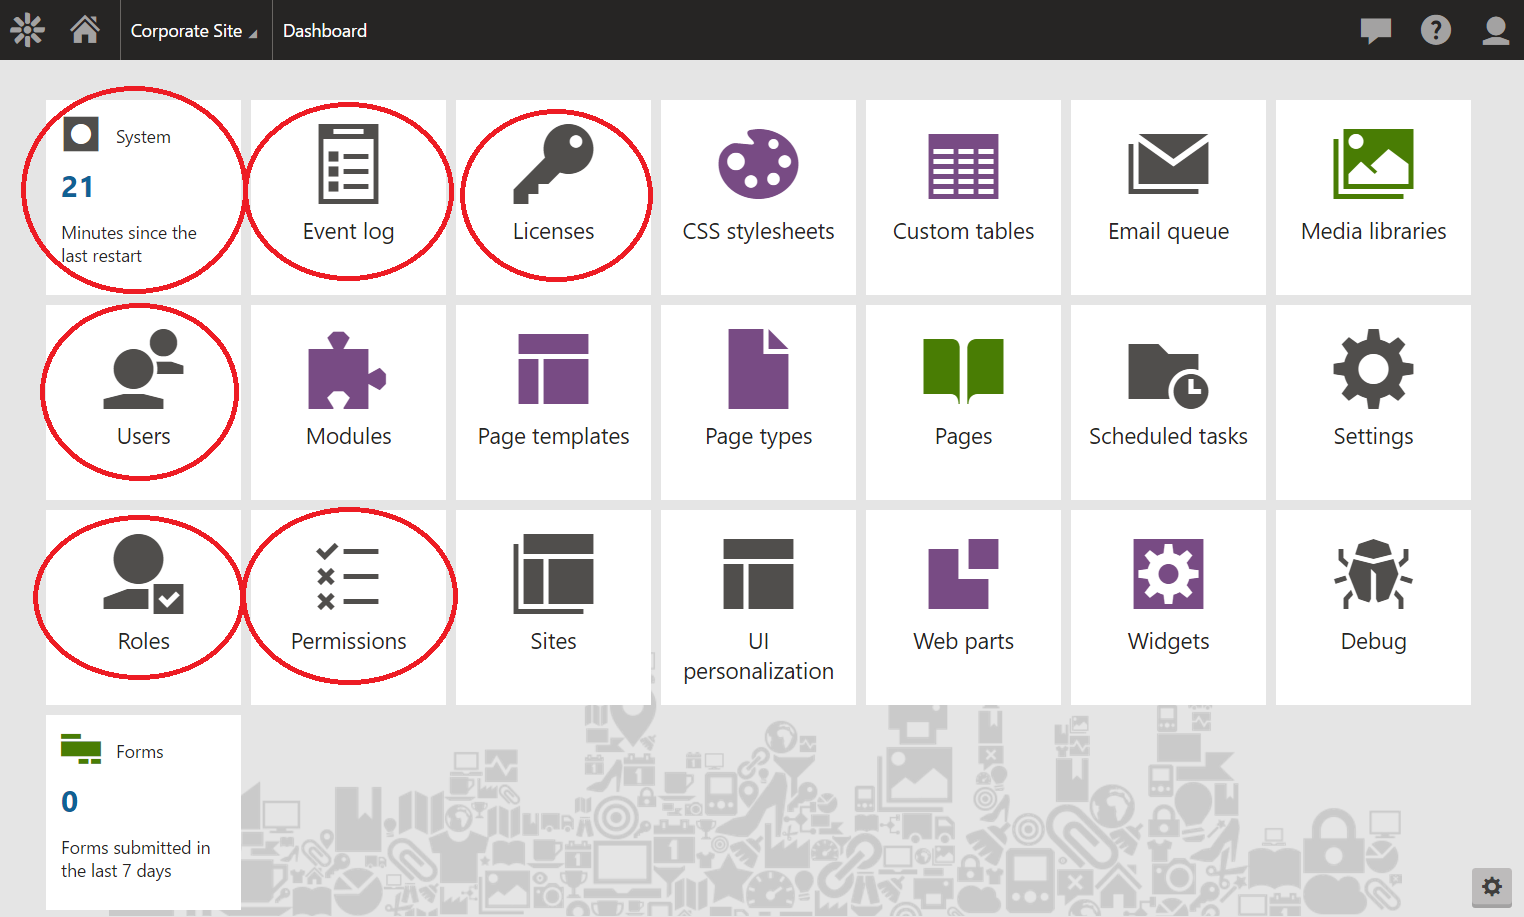
\includegraphics[width=\textwidth]{Images/Kentico9.png}
  \caption{Kentico 9.0 UI. The functionality of the tiles in the red circle is implemented in the KenticoApp. This image was
taken via print screen from the administration interface of the Kentico 9.0 product and modified for illustrational purposes.}
  \label{kentico9UI}
\end{figure} 

\begin{figure}[ht!]
  \centering
  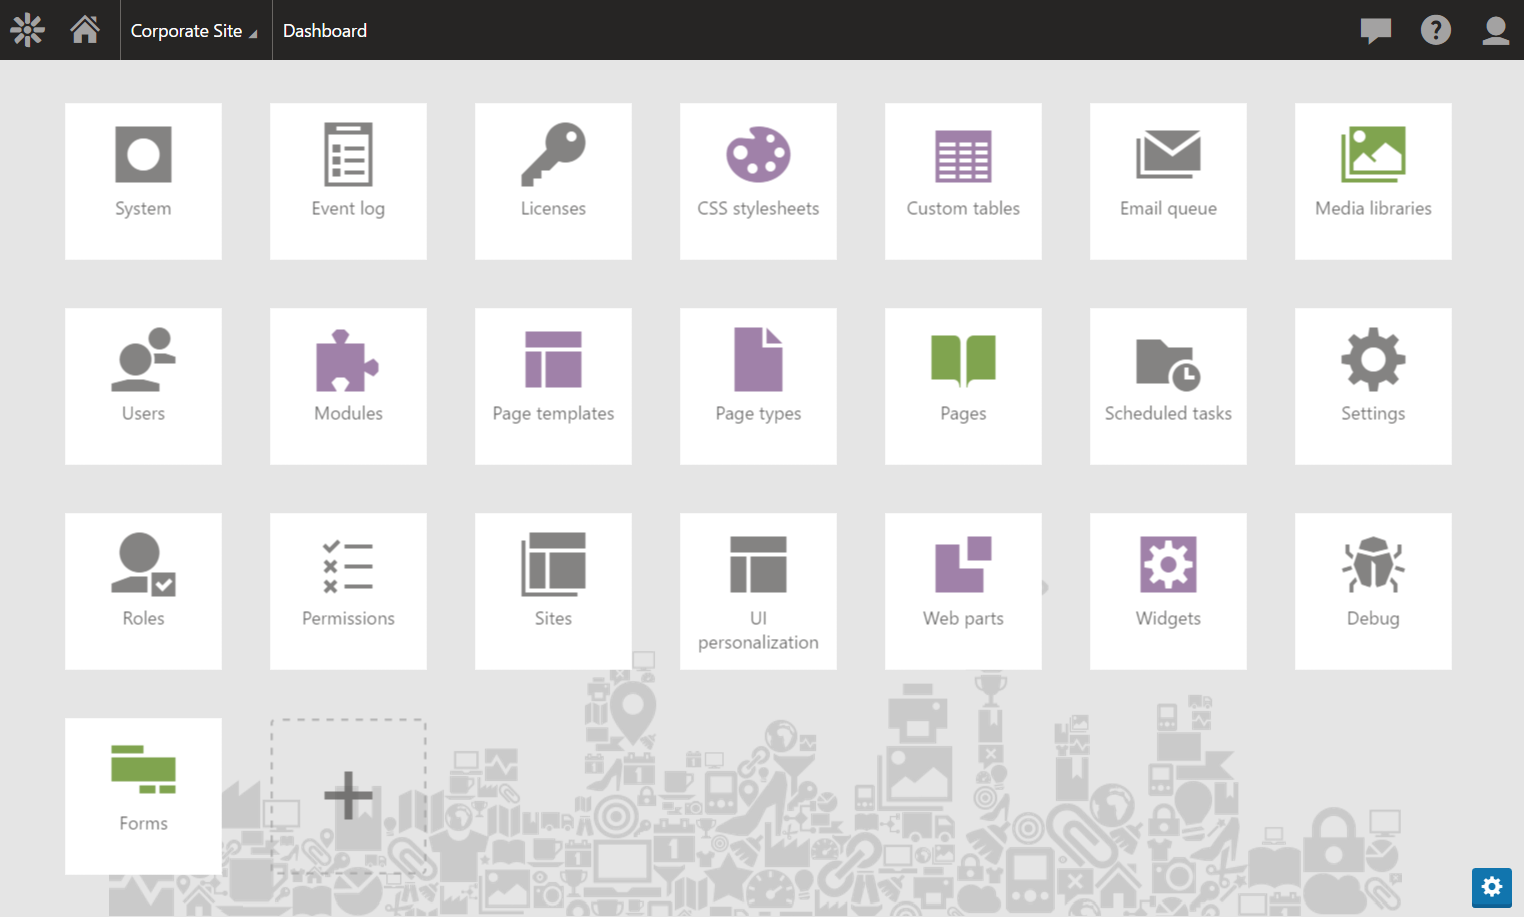
\includegraphics[width=\textwidth]{Images/Kentico9EditBtnPressed.png}
  \caption{Kentico 9.0 UI after pressing the edit button. This image was
taken via print screen from the administration interface of the Kentico 9.0 product and modified for illustrational purposes.}
  \label{kentico9UIEditBtnPressed}
\end{figure} 
\section{Web Application Interface} \label{analysisWebAPI}
\section{Hybrid Mobile application} \label{analysisHybridMobileApplication}
